%=========================================================
%  FPGA Implementation
%=========================================================
\section{FPGA Implementation}

\subsection{FPGA Configurations}

The target FPGA is the Intel MAX 10 10M50DAF484C7G and the target board is the Terasic DE10-Lite Board, as shown in Figure \ref{fig:DE10LITE}.\\

There are two configurations, as shown in Table \ref{tb:FPGACONFIG}: (1) RV32IMAC with selectable 4-wire JTAG or 2-wire cJTAG, (2) RV32IMAFC with selectable 4-wire JTAG or 2-wire cJTAG. You can select each configuration by disabling or enabling the \textasciigrave define switches: RISCV\_ISA\_RV32F in defines\_core.v, which is stored in the ./verilog/common directory.\\

If the RISC-V ISA in mmRISC-1 does not have floating point instructions (RV32IMAC: \textasciigrave define RISCV\_ISA\_RV32F is disabled), the FPGA operates at 20MHz (Tcyc = 50ns). However, if it has floating point instructions (RV32IMAFC: \textasciigrave define RISCV\_ISA\_RV32F is enabled), the FPGA operates at 16.67MHz (Tcyc = 60ns) due to the complexity of logic for floating point operations. In the CHIP\_TOP layer, if “\textasciigrave RISCV\_ISA\_RV32F” is defined, the 16.67MHz output from the PLL is used as the system clock. Otherwise, the 20MHz output from the PLL is used. The examples of FPGA configuration results are shown in Table \ref{tb:FPGACONFIG}.\\

The FPGA-related resources are stored in the directory "mmRISC-1/fpga". After launching Quartus Prime (Figure \ref{fig:QUESTAPRIME}), please open the project file "mmRISC.qpf". The timing constraints file is "mmRISC.sdc". \\

Please compile the project. Then, you will find a non-volatile MAX 10 FLASH configuration file "mmRISC.pof" and a volatile MAX 10 SRAM configuration file "mmRISC.sof" in the directory "./fpga/output\_files". Please download either of them to the FPGA via the USB Blaster Interface using the "Programmer" application of Quartus Prime.


\subsection{Initialization of Instruction RAM}

If you want to make the Instruction RAM have initial data like a ROM, apply the macro keyword "FPGA" in the Quartus synthesis setting. And place the initialization data RAM128KB\_DP.mif in the directory "fpga", which can be generated from the Intel Hex format by the hex2mif command prepared in the directory "tools" as shown below. The source code of the tool hex2mif.c is located in the same directory. A “**.hex” is an Intel Hex format binary built from your C program.\\

\texttt{\$ ./tools/hex2mif ***.hex >  RAM128KB\_DP.mif}

The macro "FPGA" switches ram.v to ram\_fpga.v for the Instruction RAM (U\_RAMI) in the chip\_top layer. The ram\_fpga.v refers to the FPGA IP of RAM128KB\_DP.v stored in the directory "fpga".\\

The already prepared RAM128KB\_DP.mif has been generated from "mmRISC\_TouchLCD" (without floating point instructions) by the above command. If there is no Touch LCD shield on the FPGA board, this demo program toggles LEDs and outputs 3D acceleration sensor data to the UART terminal.


\begin{figure}
    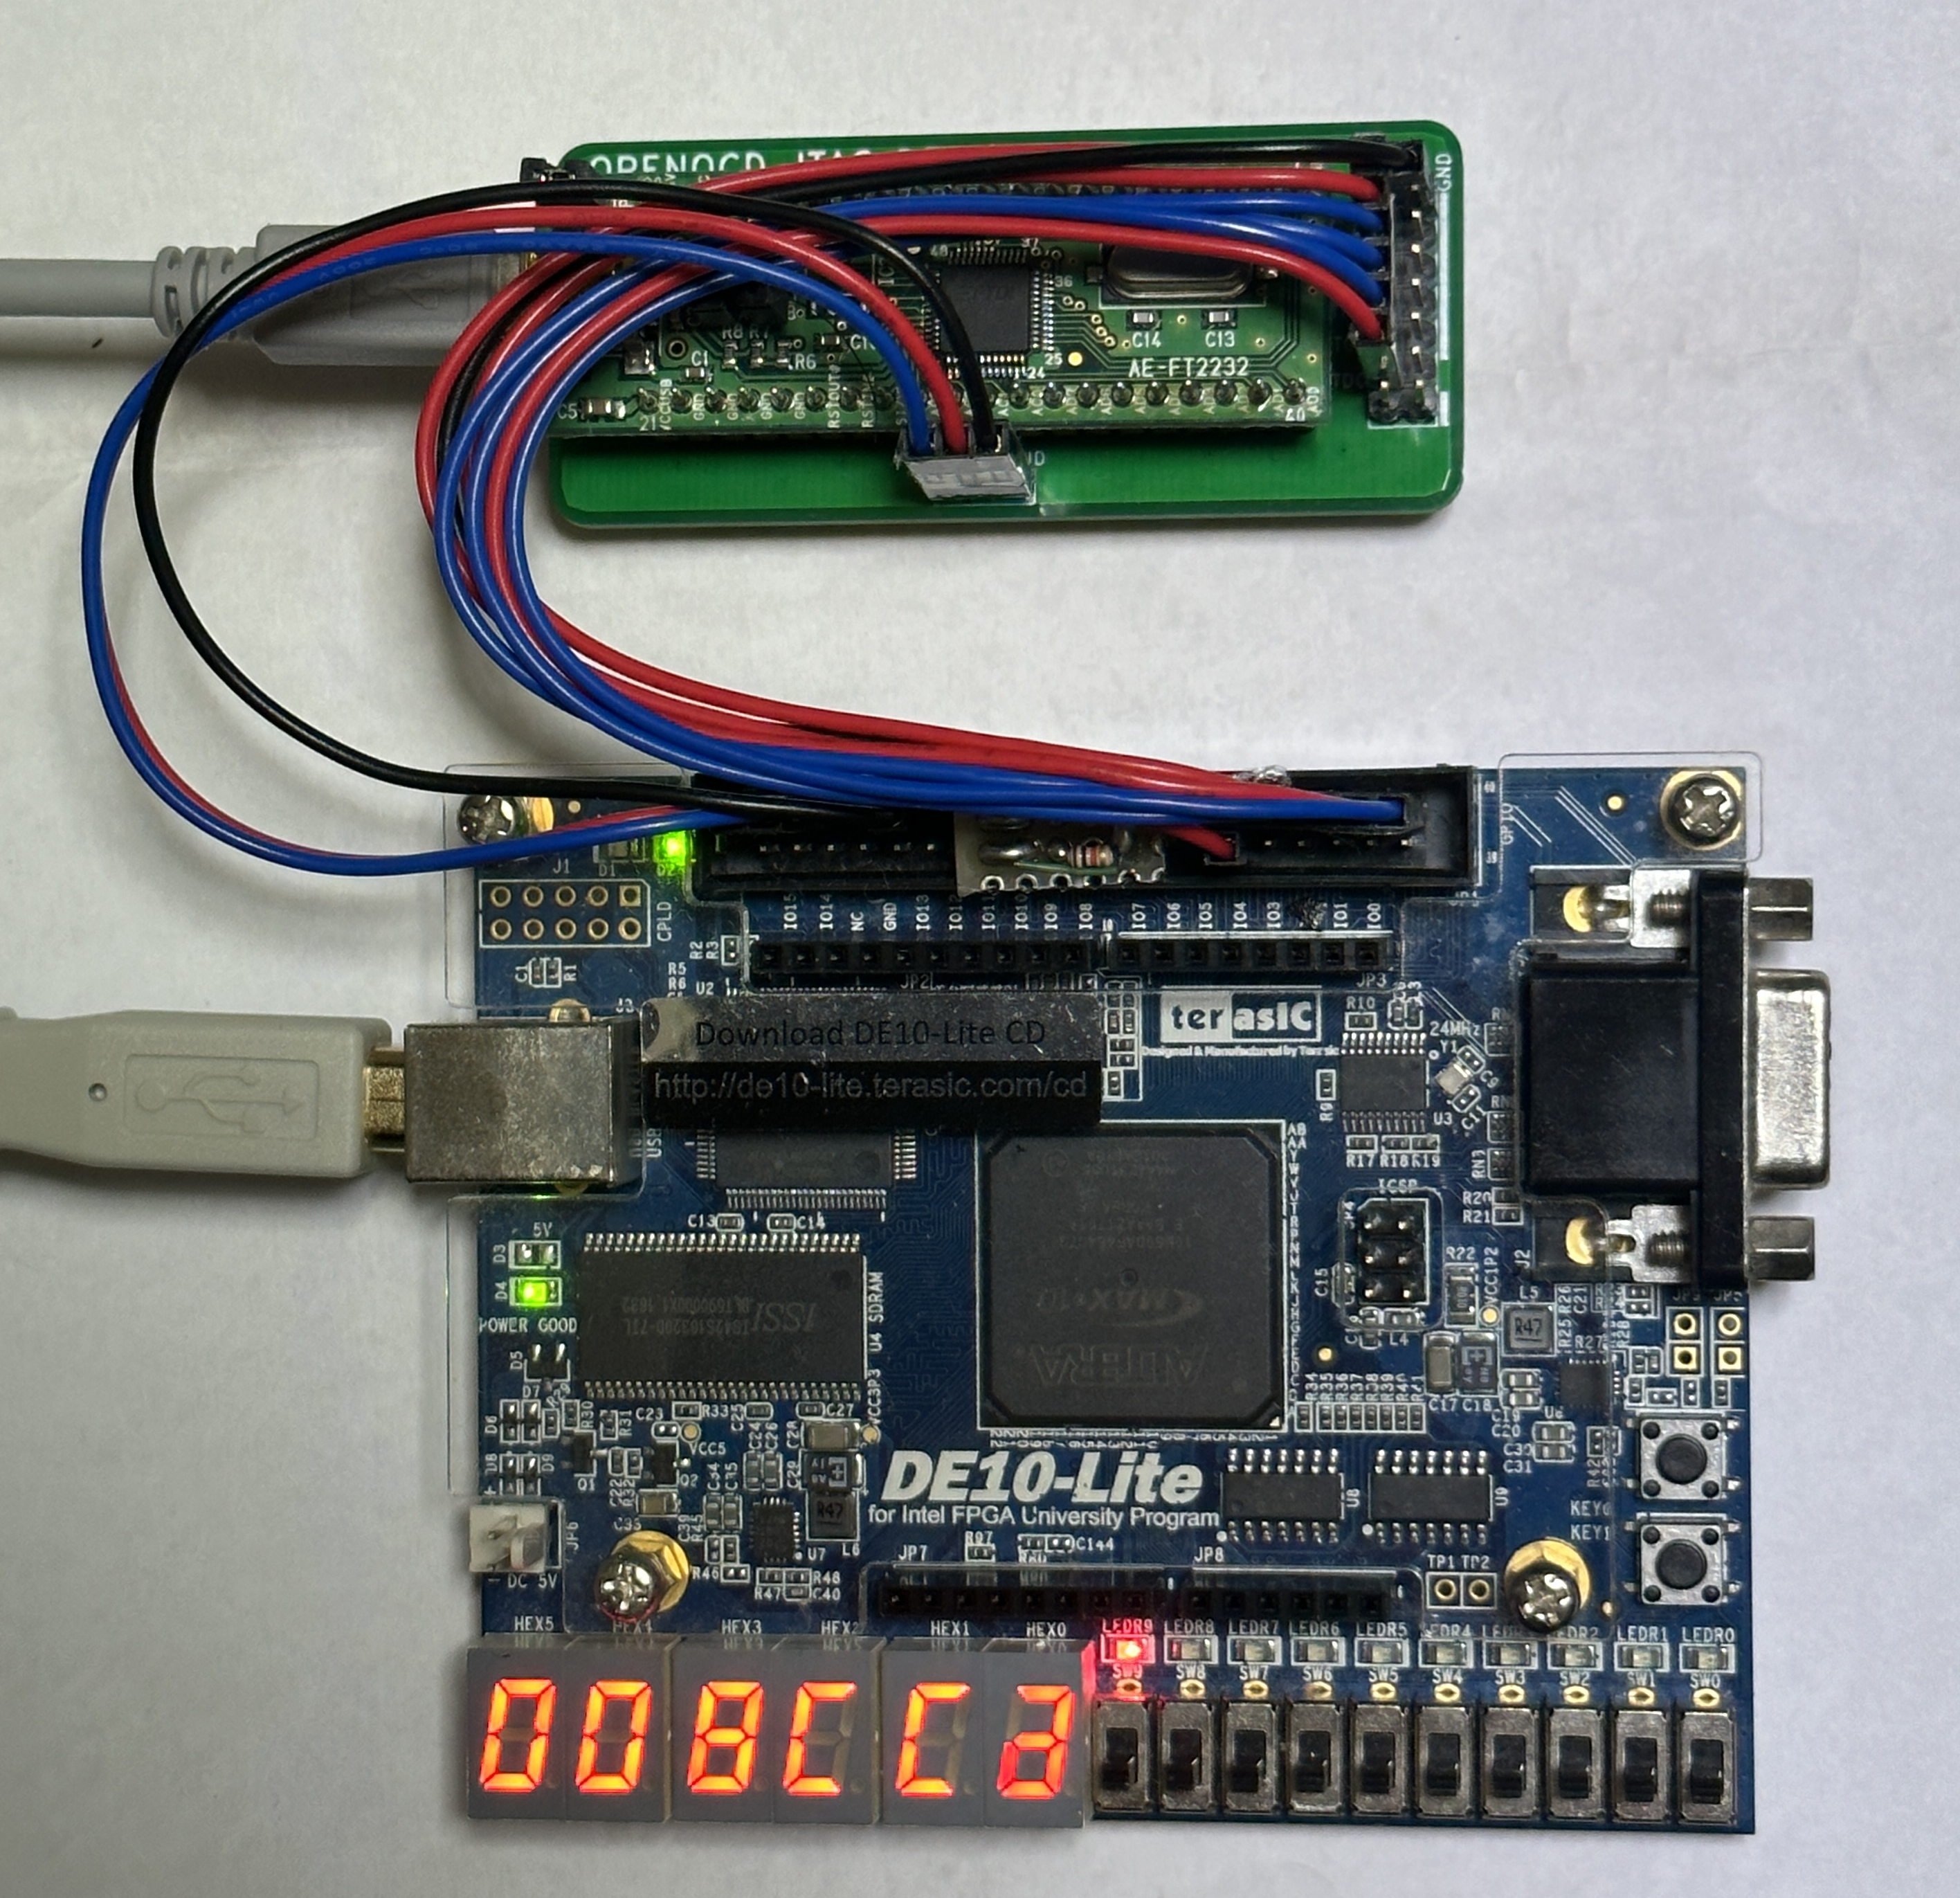
\includegraphics[width=0.8\columnwidth]{./Figure/DE10-Lite.png}
    \caption{Terasic DE10-Lite Board \& OpenOCD JTAG Adapter}
    \label{fig:DE10LITE}
\end{figure}

\begin{figure}
    \includegraphics[width=1.0\columnwidth]{./Figure/QuestaPrime.png}
    \caption{Intel Quartus Prime Lite Edition}
    \label{fig:QUESTAPRIME}
\end{figure}

\begin{table}
    \begin{adjustbox}{scale={0.95}{1}}
    \textsf{
    \begin{tabular}{|L{4cm}{4cm}{t}|L{4cm}{4cm}{t}|L{4cm}{4cm}{t}|L{1cm}{1cm}{t}|}
        \hline
        %-------------------------------------
        \rowcolor{LightPurple}
        \textbf{RISC-V ISA} &
        \textbf{RV32IMAC (integer)} &
        \textbf{RV32IMAFC (interger + floating)} &
        \textbf{Note}
        \nextRow \hline
        %-------------------------------------
        Configuration Data &
        ./fpga/output\_files/ \lb RV32IMAC\_JTAGcJTAG/\ \  \lb mmRISC.pof &
        ./fpga/output\_files/ \lb RV32IMAFC\_JTAGcJTAG/\  \lb mmRISC.pof &
        ~
        \nextRow \hline
        %-------------------------------------
        Debug I/F &
        \setMultiColumn{2}{12cm}{8cm}{l}{t}{}{|}
        {4-wire JTAG} &
        ~
        \nextRow \hline
        %-------------------------------------
        Peripherals &
        \setMultiColumn{2}{12cm}{8cm}{l}{t}{}{|}
        {Instruction RAM 128KB (initialized by .mif), \lb 
         Data RAM 48KB , Multilayer AHB BUS, \lb
         UART + Timer + GPIO + I2C(2ch) \lb 
         + SPI + SDRAM I/F} &
        ~
        \nextRow \hline
        %-------------------------------------
        Device &
        \setMultiColumn{2}{12cm}{8cm}{l}{t}{}{|}
        {MAX 10 10M50DAF484C7G} &
        ~
        \nextRow \hline
        %-------------------------------------
        Quartus Prime &
        \setMultiColumn{2}{12cm}{8cm}{l}{t}{}{|}
        {Lite Edition Ver.23.1std.0} &
        ~
        \nextRow \hline
        %-------------------------------------
        Optimization &
        \setMultiColumn{2}{12cm}{8cm}{l}{t}{}{|}
        {Performance (High effort)} &
        ~
        \nextRow \hline
        %-------------------------------------
        Logic Elements &
        25266/49760 = 49.8\% &
        43190/49760 = 86.8\% &
        ~
        \nextRow \hline
        %-------------------------------------
        Interconnect Usage &
        81,6\% (peak) &
        91.8\% (peak) &
        ~
        \nextRow \hline
        %-------------------------------------
        Frequency &
        20MHz &
        16.67MHz &
        ~
        \nextRow \hline
        %-------------------------------------
        Worst Setup Slack &
        0.964ns (met) &
        4.662ns (met) &
        ~
        \nextRow \hline
        %-------------------------------------
    \end{tabular}
    }
    \end{adjustbox}
    \caption{FPGA Configuration Results of mmRISC-1}
    \label{tb:FPGACONFIG}
\end{table}


\subsection{TIPS: How to configure the FPGA on ARM based macOS environment}

Even if your environment is an ARM-based macOS machine, such as a MacBook Pro with Apple Silicon M-series, you can install and use Intel Questa Prime on the Windows OS for 64-bit ARM on the Parallels Desktop. However, you cannot configure the FPGA via the USB Blaster cable from the ARM Windows. In such a case, please configure the FPGA from macOS by using UrJTAG and the SVF (Serial Vector Format) file.\\

\textbf{STEP 1: Convert configuration file to SVF}\\
To convert the configuration file to SVF, follow these steps:

(1) In the "Programmer" window, add the "./fpga/output\_files/mmRISC.sof" for the MAX 10 SRAM configuration (volatile) or the "./fpga/output\_files/mmRISC.pof" for the MAX 10 FLASH configuration (non-volatile).

(2) For the "mmRISC.pof", do not forget to check the box of "Program/Configure" in the "CFM0" line.

(3) Select the menu "File" --> "Create JAM, JBC, SVF, or ISC File...", and select "Serial Vector Format (.svf)" from the "File format" drop-down list.

(4) Enter the file name "mmRISC.sof.svf" to be converted from "mmRISC.sof", or the file name of "mmRISC.pof.svf" to be converted from "mmRISC.pof" in the "File name" field.

(5) The conversion will start when you click the OK button.\\

\textbf{STEP 2: Install UrJTAG on your macOS}\\
To install UrJTAG on your macOS, follow these steps:

(1) Download the UrJTAG source files from http://urjtag.org and extract the tarball.

(2) \texttt{\% ./configure}

(3) \texttt{\% make} (If you encounter a link error during the "make" process, please search for the countermeasures from the internet because they might depend on the UrJTAG versions.)

(4) \texttt{\% sudo make install}

(5) Confirm whether the "jtag" command works on the terminal window.

(6) Find and download the BSDL file "MAX\_10\_10M50DAF484.bsdl" from the internet.

(7) After launching the "jtag" command, convert the BSDL file to a JTAG information data by using the subcommand shown below in the "jtag" command session.

\texttt{jtag> bsdl dump MAX\_10\_10M50DAF484.bsdl}\\
And save the displayed data as a text file named "10M50DAF484" in /usr/local/share/urjtag/altera/10m50daf484.

(8) Quit from the "jtag" command session by using the "quit" command.

(9) You can find a text file "PARTS" in /usr/local/share/urjtag/altera. Append the following line at the bottom of the "PARTS" file.

\texttt{0011000100000101 10m50daf484 10M50DAF484}

(10) Create a text file "STEPPINGS" in /usr/local/share/urjtag/altera/10m50daf484 with the following content:

\texttt{0000 10m50daf484 0}

(11) Just for your reference, (9) and (10) are based on the following information described in the BSDL file.

\begin{lstlisting}[frame=single, language=, basicstyle=\ttfamily\scriptsize]
attribute IDCODE_REGISTER of MAX_10_10M50DAF484 : entity is
  "0000"&               --4-bit Version
  "0011000100000101"&   --16-bit Part Number
  "00001101110"&        --11-bit Manufacturer's Identity
  "1";                  --Mandatory LSB
\end{lstlisting}
\vskip\baselineskip

\textbf{STEP 3: Configure the FPGA by UrJTAG} \\
To configure the FPGA, follow these steps:

(1) Connect your FPGA board and Mac via the USB Blaster cable.

(2) Launch the "jtag" command in your terminal.

(3) In the "jtag" session, enter the "cable" command as follows.

\texttt{jtag> cable UsbBlaster}

(4) Enter the "detect" command as follows.
\texttt{jtag> detect}\\
If successful, you will see the following messages.
\begin{lstlisting}[frame=single, language=, basicstyle=\ttfamily\scriptsize]
IR length: 10
Chain length: 1
Device Id: 00000011000100000101000011011101 (0x031050DD)
  Manufacturer: Altera (0x0DD)
  Part(0):      10M50DAF484 (0x3105)
  Stepping:     0
  Filename:     /usr/local/share/urjtag/altera/10m50daf484/10m50daf484}
\end{lstlisting}

(5) Program the FPGA by using the SVF. For the MAX 10 SRAM configuration (volatile):\\
\texttt{jtag> svf mmRISC.sof.svf stop progress}\\
For the MAX 10 FLASH configuration (non-volatile):\\
\texttt{jtag> svf mmRISC.pof.svf stop progress}

(6) Quit from the “jtag” command.


\subsection{FPGA Pin Assignments}

The FPGA pin assignments are shown in Table \ref{tb:FPGAPIN1} and Table \ref{tb:FPGAPIN2}. The Table \ref{tb:FPGAPINSPECIAL} shows some pins for special functions of the mmRISC-1 tiny SoC, such as cJTAG, stand-by (low power mode), authentication (security), slow clock, and halt-on-reset, which are described in Section \ref{sec:MISCELLANEOUS}. The positions on the FPGA board to use the special features are shown in Figure \ref{fig:SPECIALFEATURES}.


\begin{table}[H]
    \includegraphics[width=1.0\columnwidth]{./Table/FPGAPinAssign1.png}
    \caption{FPGA Pin Assignments (1)}
    \label{tb:FPGAPIN1}
\end{table}

\begin{table}[H]
    \includegraphics[width=1.0\columnwidth]{./Table/FPGAPinAssign2.png}
    \caption{FPGA Pin Assignments (2)}
    \label{tb:FPGAPIN2}
\end{table}

\begin{table}[H]
    \includegraphics[width=1.0\columnwidth]{./Table/FPGASpecialPin.png}
    \caption{FPGA Special Function Pins}
    \label{tb:FPGAPINSPECIAL}
\end{table}

\begin{figure}[H]
    \includegraphics[width=1.0\columnwidth]{./Figure/SpecialFeatures.png}
    \caption{Operation Positions to use special features}
    \label{fig:SPECIALFEATURES}
\end{figure}


